\documentclass[11pt]{beamer}
% \usetheme{Boadilla}
  \usetheme{default}


% acronyms for text or math mode
\newcommand {\ccast} {\mbox{\small CCAST}}
\newcommand {\cris} {\mbox{\small CrIS}}

\newcommand {\airs} {\mbox{\small AIRS}}
\newcommand {\iasi} {\mbox{\small IASI}}
\newcommand {\idps} {\mbox{\small IDPS}}
\newcommand {\nasa} {\mbox{\small NASA}}
\newcommand {\noaa} {\mbox{\small NOAA}}
\newcommand {\nstar} {\mbox{\small STAR}}
\newcommand {\umbc} {\mbox{\small UMBC}}
\newcommand {\uw}   {\mbox{\small UW}}

\newcommand {\fft}  {\mbox{\small FFT}}
\newcommand {\ifft} {\mbox{\small IFFT}}
\newcommand {\fir}  {\mbox{\small FIR}}
\newcommand {\fov}  {\mbox{\small FOV}}
\newcommand {\for}  {\mbox{\small FOR}}
\newcommand {\ict}  {\mbox{\small ICT}}
\newcommand {\ils}  {\mbox{\small ILS}}
\newcommand {\igm}  {\mbox{\small IGM}}
\newcommand {\opd}  {\mbox{\small OPD}}
\newcommand {\rms}  {\mbox{\small RMS}}
\newcommand {\zpd}  {\mbox{\small ZPD}}
\newcommand {\ppm}  {\mbox{\small PPM}}
\newcommand {\srf}  {\mbox{\small SRF}}
\newcommand {\sdr}  {\mbox{\small SDR}}

\newcommand {\ES} {\mbox{\small ES}}
\newcommand {\SP} {\mbox{\small SP}}
\newcommand {\IT} {\mbox{\small IT}}
\newcommand {\SA} {\mbox{\small SA}}

\newcommand {\ET} {\mbox{\small ET}}
\newcommand {\FT} {\mbox{\small FT}}

% abbreviations, mainly for math mode
\newcommand {\real} {\mbox{real}}
\newcommand {\imag} {\mbox{imag}}
\newcommand {\atan} {\mbox{atan}}
\newcommand {\obs}  {\mbox{obs}}
\newcommand {\calc} {\mbox{calc}}
\newcommand {\sinc} {\mbox{sinc}}
\newcommand {\psinc} {\mbox{psinc}}
\newcommand {\std} {\mbox{std}}

% symbols, for math mode only
\newcommand {\wnum} {\mbox{cm$^{-1}$}}
\newcommand {\lmax} {L_{\mbox{\tiny max}}}
\newcommand {\vmax} {V_{\mbox{\tiny max}}}

\newcommand {\tauobs} {\tau_{\mbox{\tiny obs}}}
\newcommand {\taucal} {\tau_{\mbox{\tiny calc}}}
\newcommand {\Vdc}  {V_{\mbox{\tiny DC}}}

\newcommand {\rIT} {r_{\mbox{\tiny\textsc{ict}}}}
\newcommand {\rES} {r_{\mbox{\tiny\textsc{es}}}}
\newcommand {\robs} {r_{\mbox{\tiny obs}}}

\newcommand {\rITobs} {r_{\mbox{\tiny\textsc{ict}}}^{\mbox{\tiny obs}}}
\newcommand {\rITcal} {r_{\mbox{\tiny\textsc{ict}}}^{\mbox{\tiny cal}}}

\newcommand {\ITmean} {\langle\mbox{\small IT}\rangle}
\newcommand {\SPmean} {\langle\mbox{\small SP}\rangle}


\title{ccast and noaa \\
  relative fov response}
\author{H.~E.~Motteler, L.~L.~Strow}
\institute{
  UMBC Atmospheric Spectroscopy Lab \\
  Joint Center for Earth Systems Technology \\
}
\date{\today}
\begin{document}

%----------- slide --------------------------------------------------%
\begin{frame}[plain]
\titlepage
\end{frame}
%----------- slide --------------------------------------------------%
\begin{frame}
\frametitle{test methods}

\begin{itemize}

  \item start with \ccast\ and \noaa\ high res data from 6--8 Dec 2014

  \item take the average and standard deviation of \for\ 15 and 16
    independently for each \fov, and compare these values with the
    values for \fov\ 5

  \item results shown here are for 32,186 \ccast\ and 32,120 {\noaa}
    descending {\for}s

  \item as a precaution, {\for}s where any LW channel was greater than
    320K were discarded

  \item the intent is to show variation among {\fov}s, as might arise
    from varying nonlinearity or artifacts of the self-apodization
    correction

\end{itemize}

\end{frame}
%----------- slide --------------------------------------------------%
\begin{frame}
\frametitle{ccast LW mean}

\begin{center}
  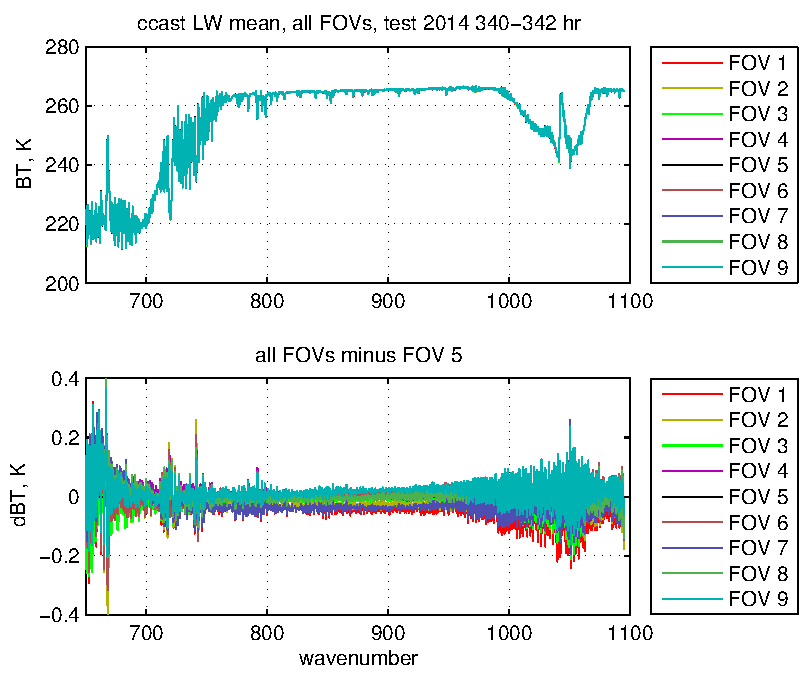
\includegraphics[scale=0.7]{figures/ccast_LW_avg_2014_340-342_hr.pdf}
\end{center}

\end{frame}
%----------- slide --------------------------------------------------%
\begin{frame}
\frametitle{noaa LW mean}

\begin{center}
  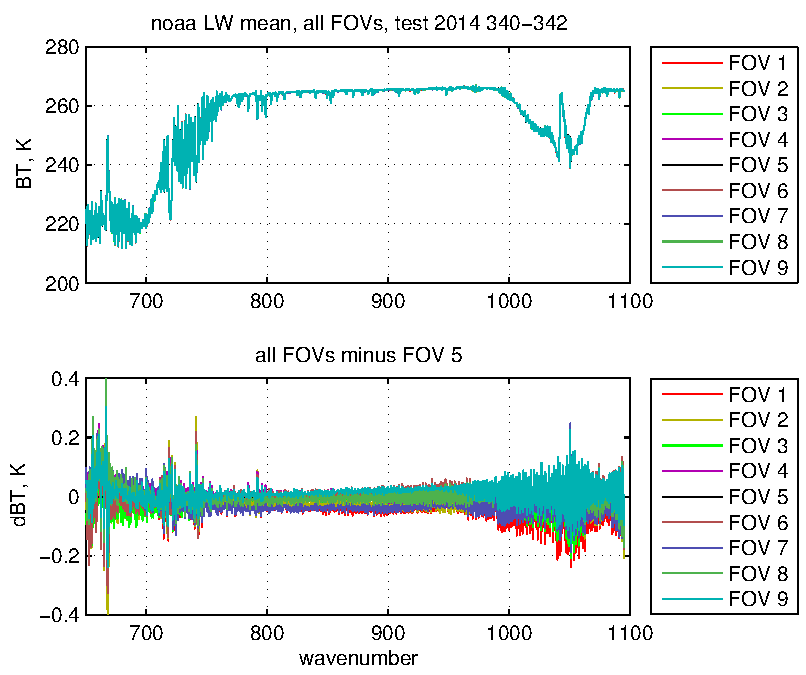
\includegraphics[scale=0.7]{figures/noaa_LW_avg_2014_340-342.pdf}
\end{center}

\end{frame}
%----------- slide --------------------------------------------------%
\begin{frame}
\frametitle{ccast LW fov groups}

\begin{center}
  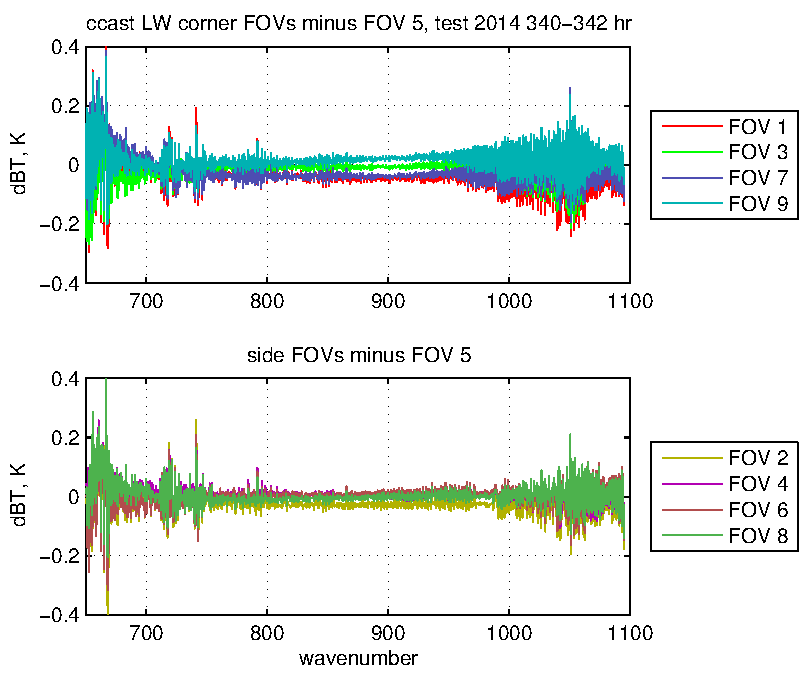
\includegraphics[scale=0.7]{figures/ccast_LW_dif_2014_340-342_hr.pdf}
\end{center}

\end{frame}
%----------- slide --------------------------------------------------%
\begin{frame}
\frametitle{noaa LW fov groups}

\begin{center}
  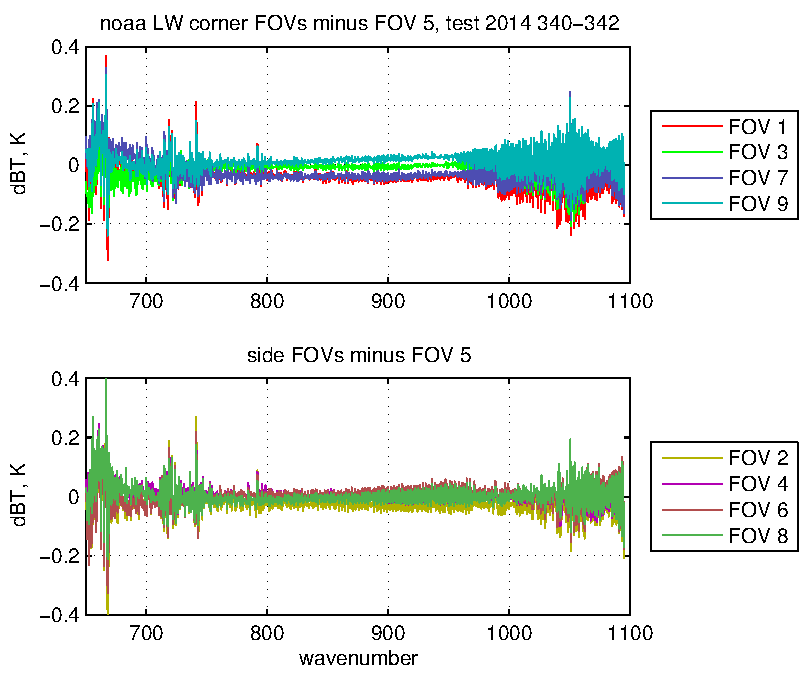
\includegraphics[scale=0.7]{figures/noaa_LW_dif_2014_340-342.pdf}
\end{center}

\end{frame}
%----------- slide --------------------------------------------------%
\begin{frame}
\frametitle{ccast minus noaa fovs 1, 2, and 5}

\begin{center}
  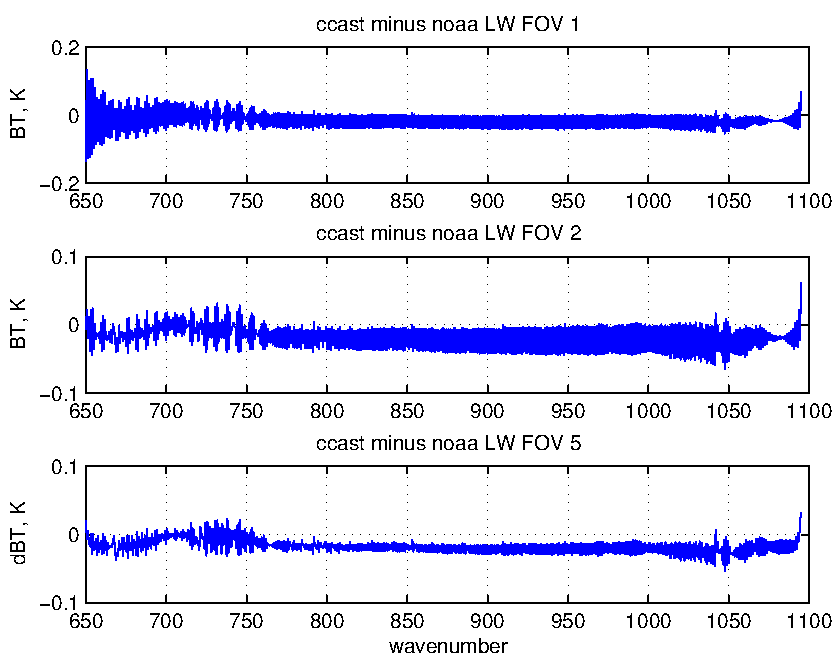
\includegraphics[scale=0.7]{figures/ccast_noaa_LW_fig_1.pdf}
\end{center}

\end{frame}
%----------- slide --------------------------------------------------%
\begin{frame}
\frametitle{ccast minus noaa fov groups}

\begin{center}
  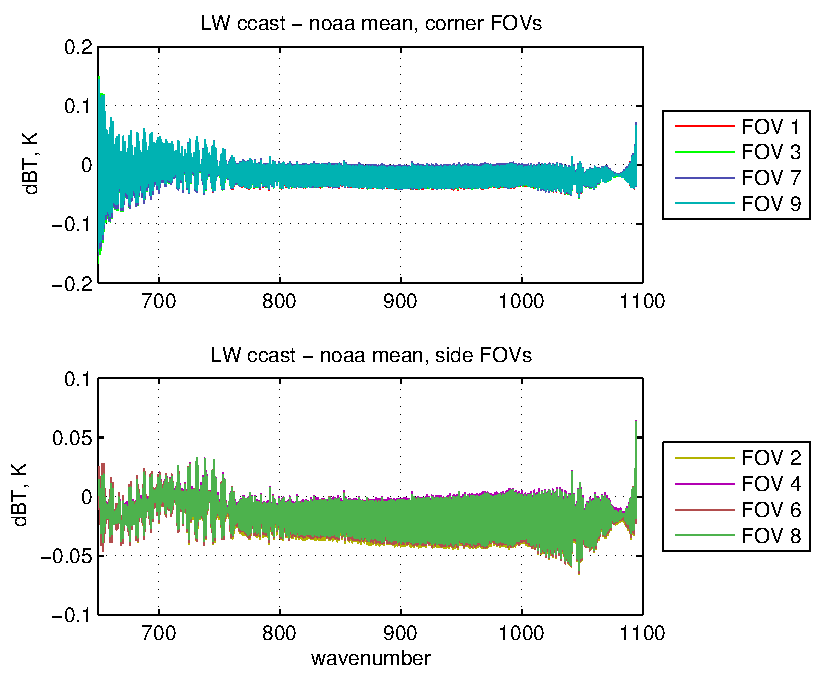
\includegraphics[scale=0.7]{figures/ccast_noaa_LW_fig_2.pdf}
\end{center}

\end{frame}
%----------- slide --------------------------------------------------%
\begin{frame}
\frametitle{ccast minus noaa relative fov groups}

\begin{center}
  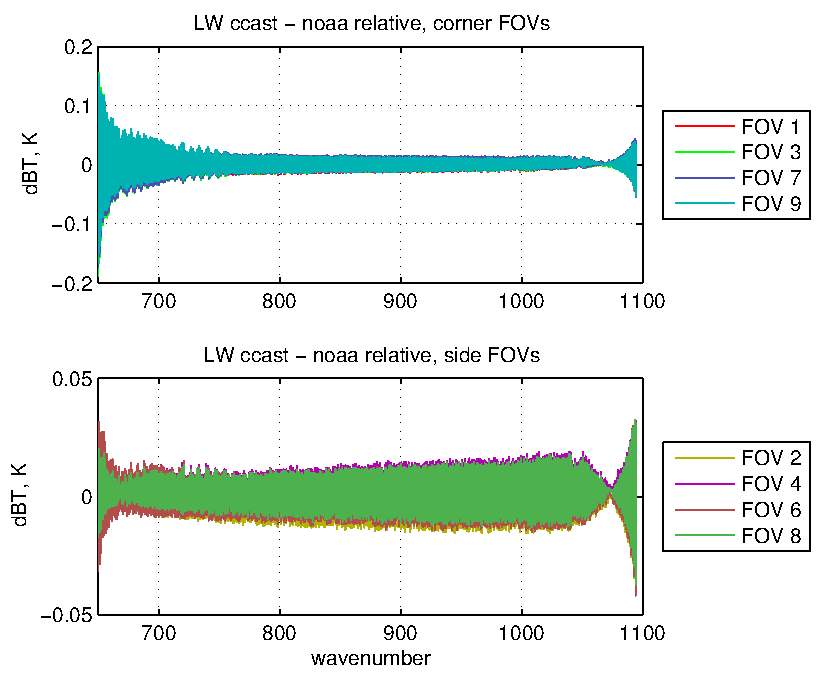
\includegraphics[scale=0.7]{figures/ccast_noaa_LW_fig_3.pdf}
\end{center}

\end{frame}
%----------- slide --------------------------------------------------%
\begin{frame}
\frametitle{LW discussion}

\begin{itemize}

  \item \ccast\ and \noaa\ are generally in good agreement

  \item in the LW, \ccast\ is around $0.02$K colder than \noaa

  \item in the previous slide, ``ccast minus noaa relative'' is \\
    (ccast all \fov s $-$ \fov\ 5) $-$ (noaa all \fov s $-$ \fov\ 5)

  \item the \ccast\ nonlinearity correction uses the UW a2 values

  \item the slightly greater difference for the corner {\fov}s at the
    low end of the band may be due to different processing filters

\end{itemize}

\end{frame}
%----------- slide --------------------------------------------------%
\begin{frame}
\frametitle{ccast MW mean}

\begin{center}
  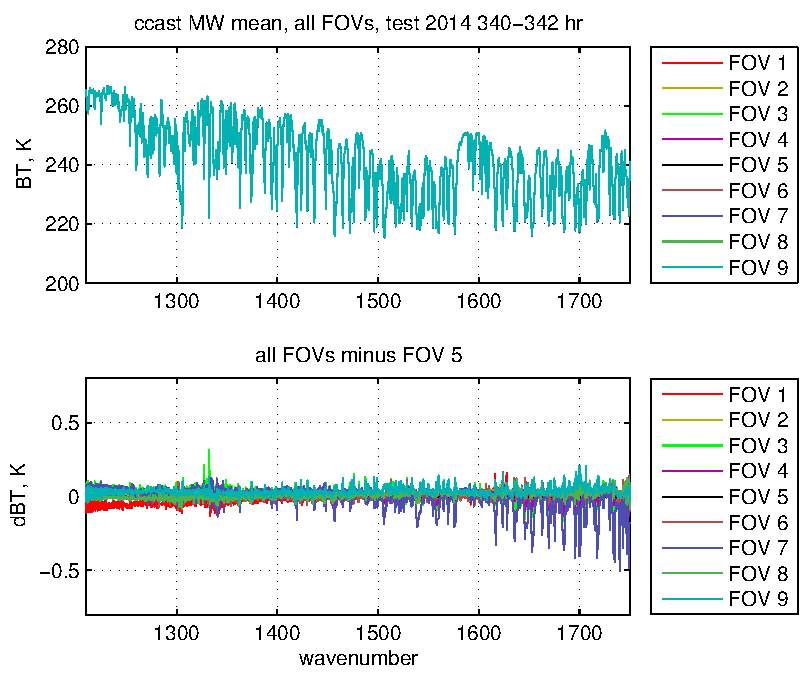
\includegraphics[scale=0.7]{figures/ccast_MW_avg_2014_340-342_hr.pdf}
\end{center}

\end{frame}
%----------- slide --------------------------------------------------%
\begin{frame}
\frametitle{noaa MW mean}

\begin{center}
  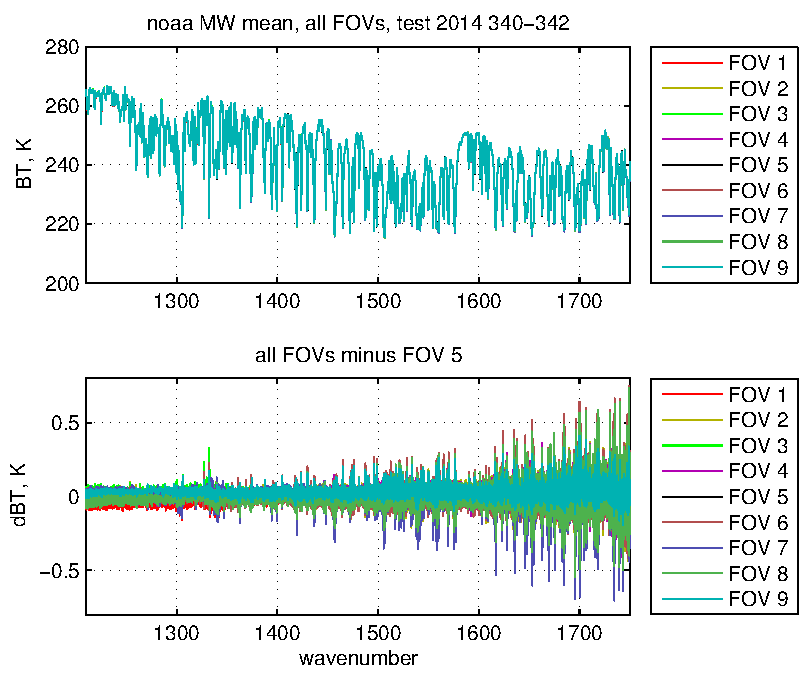
\includegraphics[scale=0.7]{figures/noaa_MW_avg_2014_340-342.pdf}
\end{center}

\end{frame}
%----------- slide --------------------------------------------------%
\begin{frame}
\frametitle{ccast MW fov groups}

\begin{center}
  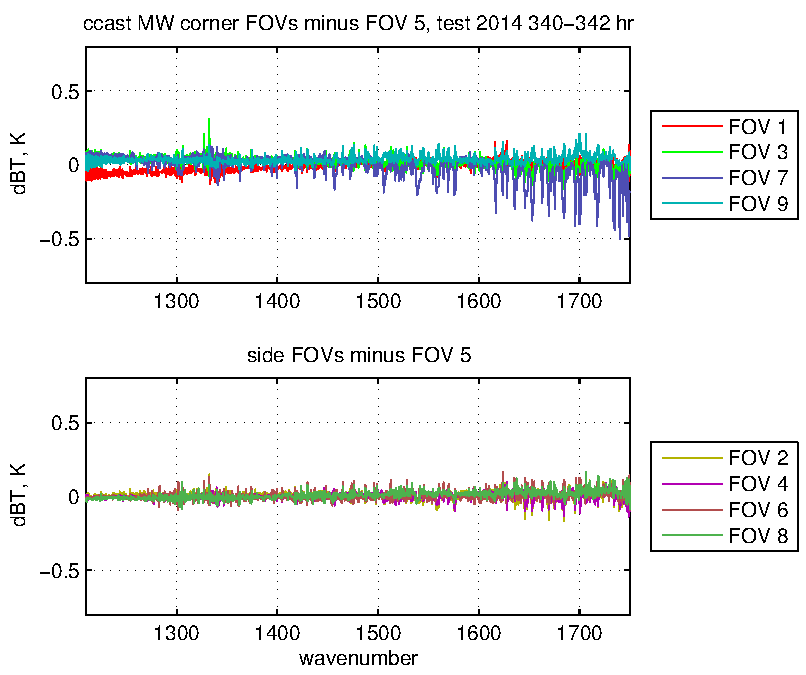
\includegraphics[scale=0.7]{figures/ccast_MW_dif_2014_340-342_hr.pdf}
\end{center}

\end{frame}
%----------- slide --------------------------------------------------%
\begin{frame}
\frametitle{noaa MW fov groups}

\begin{center}
  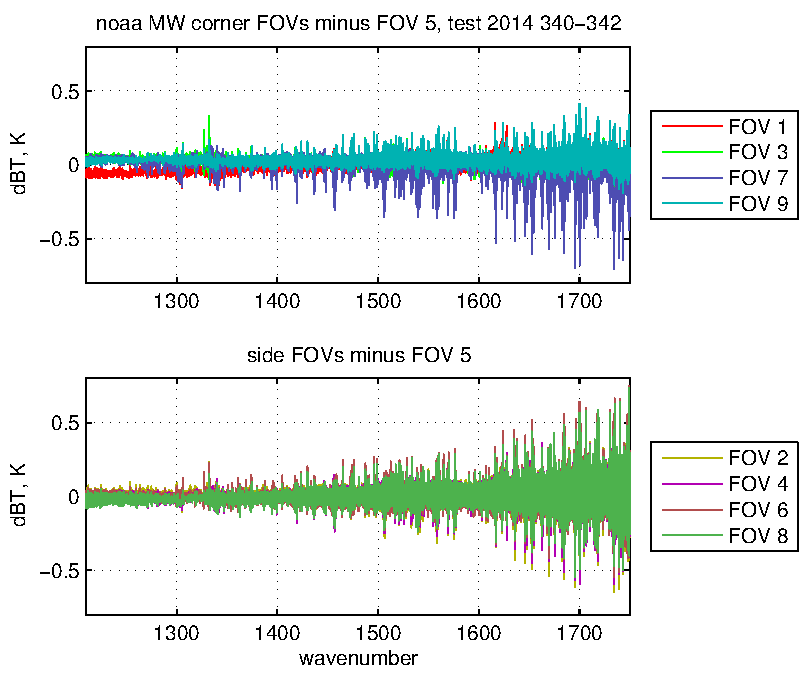
\includegraphics[scale=0.7]{figures/noaa_MW_dif_2014_340-342.pdf}
\end{center}

\end{frame}
%----------- slide --------------------------------------------------%
\begin{frame}
\frametitle{ccast minus noaa fovs 1, 2, and 5}

\begin{center}
  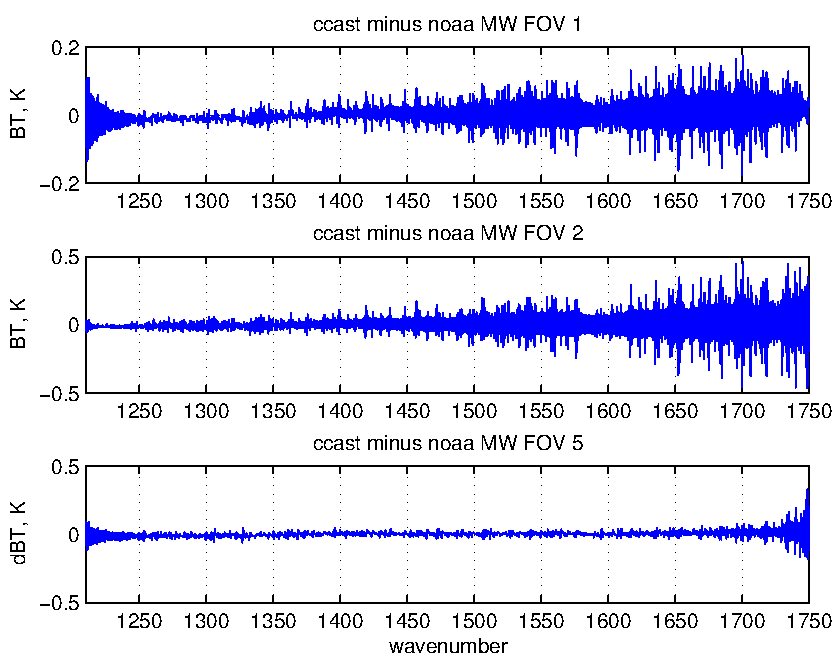
\includegraphics[scale=0.7]{figures/ccast_noaa_MW_fig_1.pdf}
\end{center}

\end{frame}
%----------- slide --------------------------------------------------%
\begin{frame}
\frametitle{ccast minus noaa fov groups}


\begin{center}
  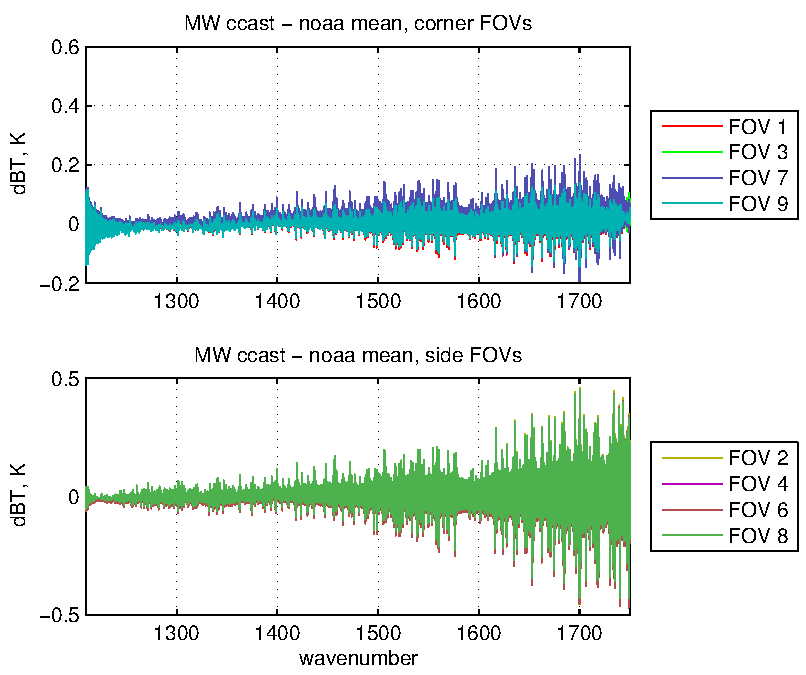
\includegraphics[scale=0.7]{figures/ccast_noaa_MW_fig_2.pdf}
\end{center}

\end{frame}
%----------- slide --------------------------------------------------%
\begin{frame}
\frametitle{ccast MW standard deviation}

\begin{center}
  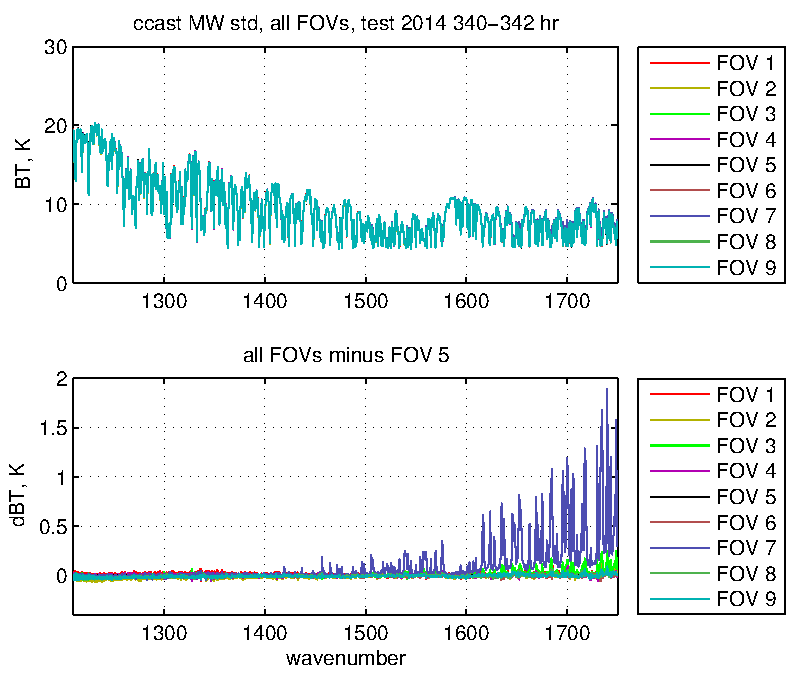
\includegraphics[scale=0.7]{figures/ccast_MW_std_2014_340-342_hr.pdf}
\end{center}

\end{frame}
%----------- slide --------------------------------------------------%
\begin{frame}
\frametitle{MW discussion}

\begin{itemize}

  \item \fov\ 7 is the least linear, and only partially corrected
    for with the \ccast\ first order adjustment

  \item the \noaa\ variation in \fov\ response is much greater than
    {\ccast}

  \item this may be due to problems with the nonlinearity correction

  \item a normalized frequency domain representation of the numeric
    filter needs a scaling factor to match the original nonlinearity
    measurements.  We used 1.6047 for LW, 0.9826 for MW, and 0.2046
    for SW

\end{itemize}

\end{frame}
%----------- slide --------------------------------------------------%
\begin{frame}
\frametitle{ccast SW mean}

\begin{center}
  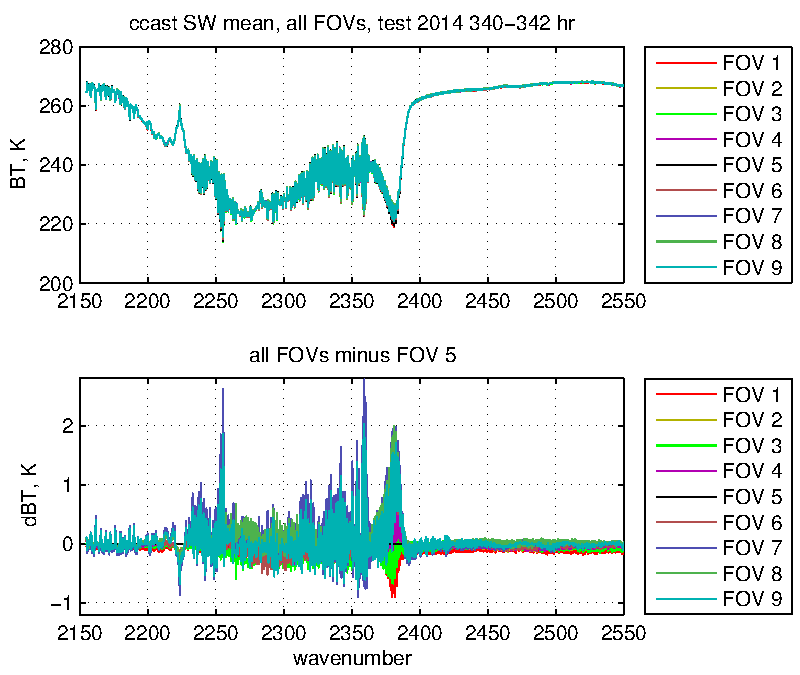
\includegraphics[scale=0.7]{figures/ccast_SW_avg_2014_340-342_hr.pdf}
\end{center}

\end{frame}
%----------- slide --------------------------------------------------%
\begin{frame}
\frametitle{noaa SW mean}

\begin{center}
  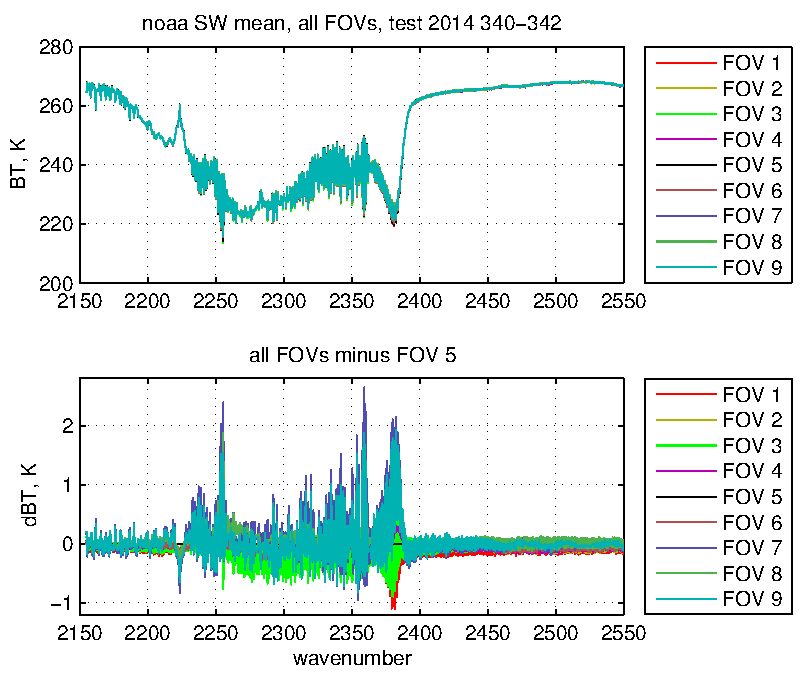
\includegraphics[scale=0.7]{figures/noaa_SW_avg_2014_340-342.pdf}
\end{center}

\end{frame}
%----------- slide --------------------------------------------------%
\begin{frame}
\frametitle{ccast SW fov groups}

\begin{center}
  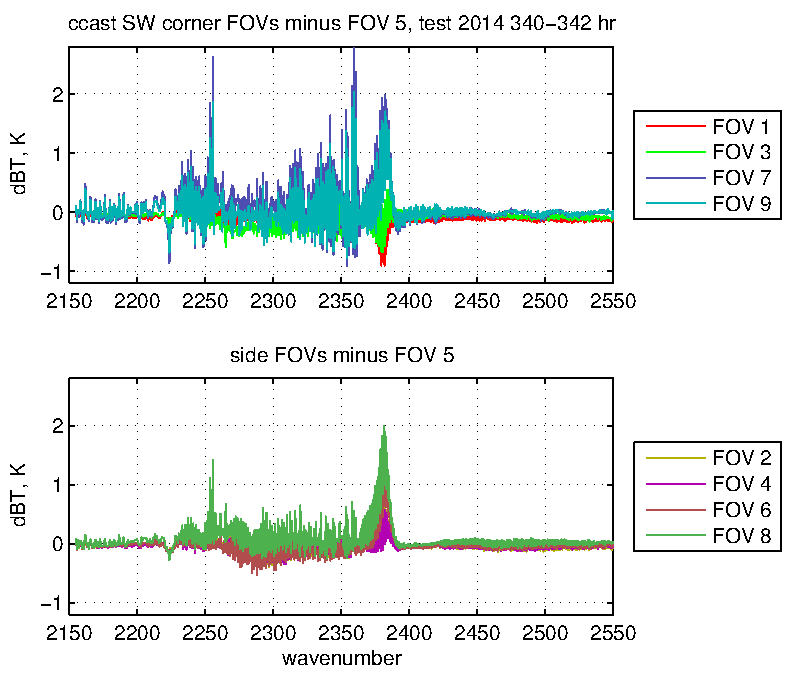
\includegraphics[scale=0.7]{figures/ccast_SW_dif_2014_340-342_hr.pdf}
\end{center}

\end{frame}
%----------- slide --------------------------------------------------%
\begin{frame}
\frametitle{noaa SW fov groups}

\begin{center}
  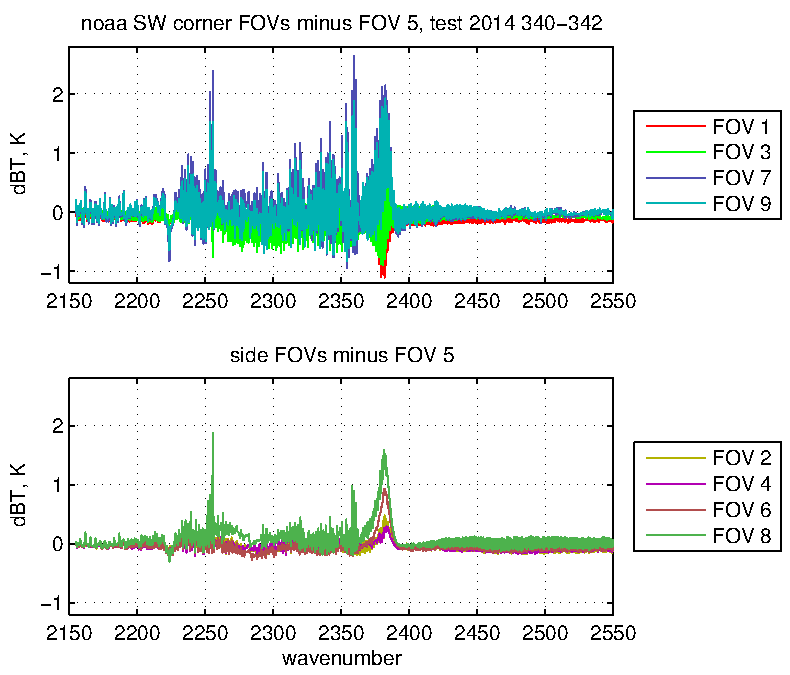
\includegraphics[scale=0.7]{figures/noaa_SW_dif_2014_340-342.pdf}
\end{center}

\end{frame}
%----------- slide --------------------------------------------------%
\begin{frame}
\frametitle{ccast minus noaa fovs 1, 2, and 5}

\begin{center}
  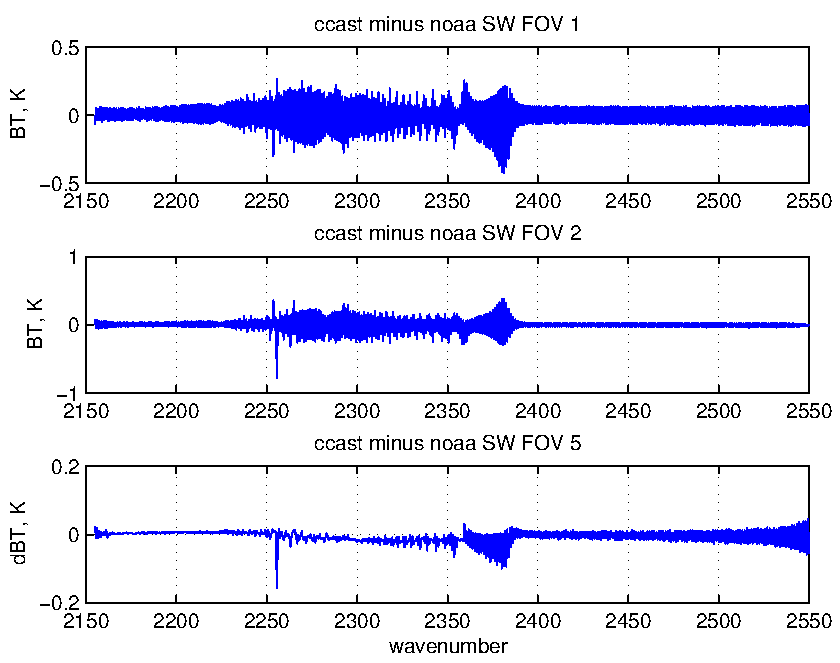
\includegraphics[scale=0.7]{figures/ccast_noaa_SW_fig_1.pdf}
\end{center}

\end{frame}
%----------- slide --------------------------------------------------%
\begin{frame}
\frametitle{ccast minus noaa fov groups}


\begin{center}
  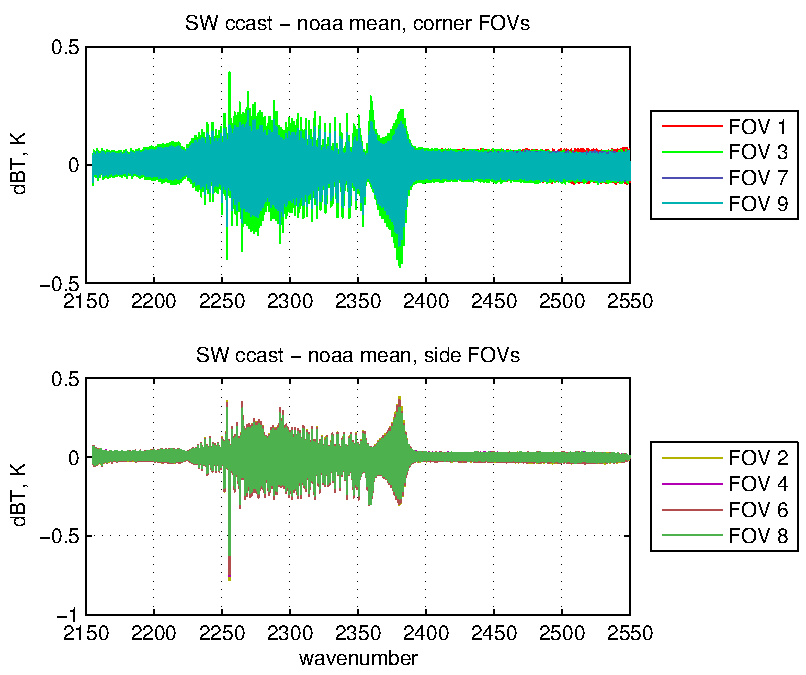
\includegraphics[scale=0.7]{figures/ccast_noaa_SW_fig_2.pdf}
\end{center}

\end{frame}
%----------- slide --------------------------------------------------%
\begin{frame}
\frametitle{SW discussion}

\begin{itemize}

  \item \ccast\ and \noaa\ are generally in good agreement

  \item residuals are significantly larger than for the LW band

  \item residuals and \noaa\ vs \ccast\ differences are generally
    greatest for the coldest lines and regions

  \item \fov\ 7 minus \fov\ 5 is significantly greater than for other
    \fov s at 2255 and 2359 \wnum, for both \ccast\ and \noaa

\end{itemize}

\end{frame}
%----------- slide --------------------------------------------------%
\begin{frame}
\frametitle{conclusions}

\begin{itemize}

  \item there is significant convergence in the \ccast\ and
    \noaa\ processing

  \item variation due to nonlinearity, especially for the MW band, is
    significantly greater than some of the more subtle effects we have
    been considering recently

  \item note again that these results are relative to \fov\ 5 or are
    direct \noaa\ vs \ccast\ comparisons, and not comparisons with
    with expected observed radiance from model data or radiance from
    other sounders

  \vspace{6mm}

  \item supplementary slides
    \begin{itemize}
      \item a comparison of standard deviations
      \item \ccast\ ILS and calibration equations
    \end{itemize}
\end{itemize}

\end{frame}
%----------- slide --------------------------------------------------%
%----------- slide --------------------------------------------------%
\begin{frame}
\frametitle{ccast LW std}

\begin{center}
  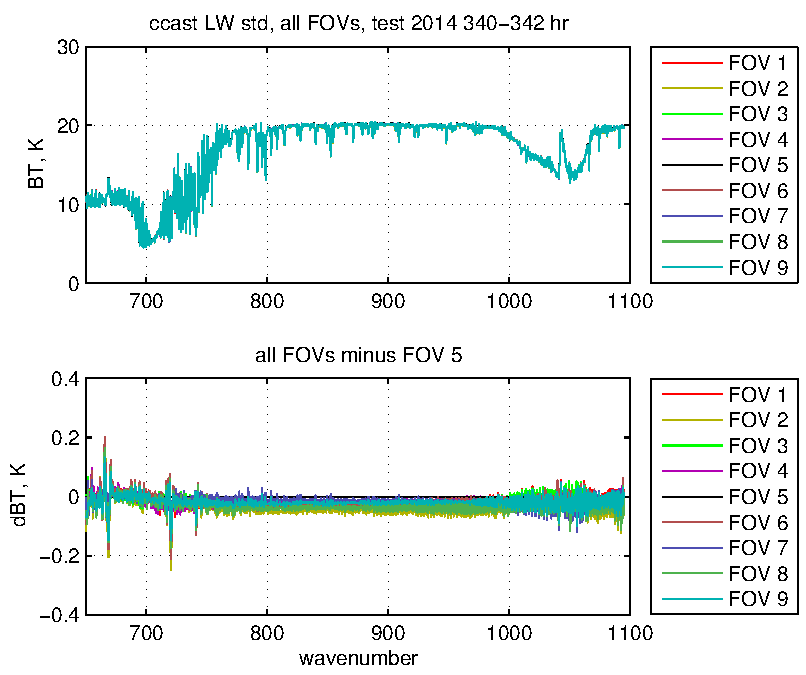
\includegraphics[scale=0.7]{figures/ccast_LW_std_2014_340-342_hr.pdf}
\end{center}

\end{frame}
%----------- slide --------------------------------------------------%
\begin{frame}
\frametitle{noaa LW std}

\begin{center}
  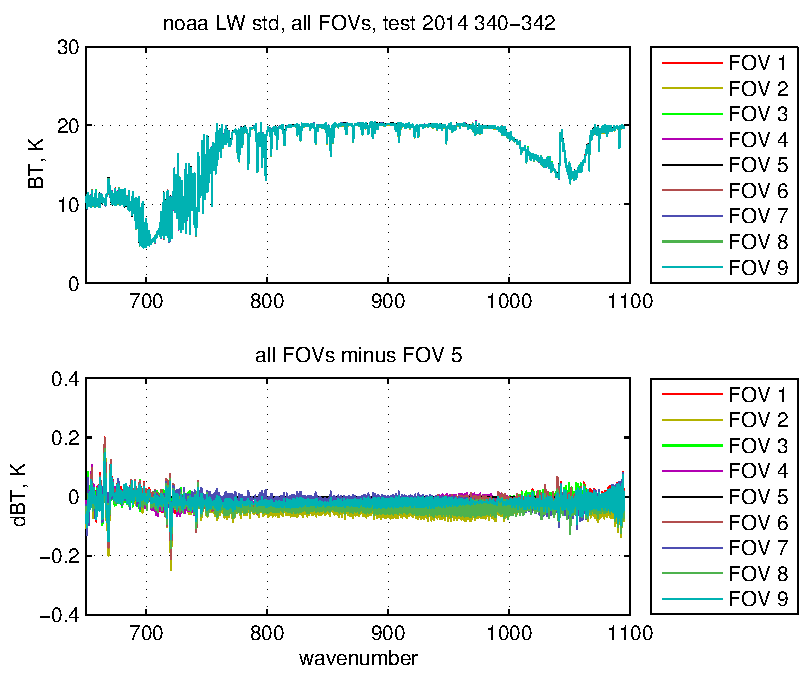
\includegraphics[scale=0.7]{figures/noaa_LW_std_2014_340-342.pdf}
\end{center}

\end{frame}
%----------- slide --------------------------------------------------%
\begin{frame}
\frametitle{ccast MW std}

\begin{center}
  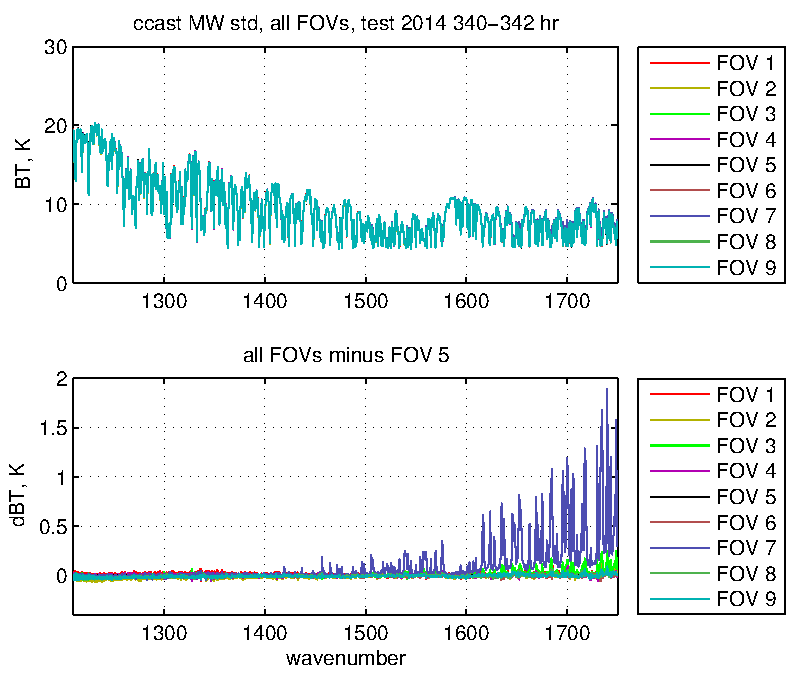
\includegraphics[scale=0.7]{figures/ccast_MW_std_2014_340-342_hr.pdf}
\end{center}

\end{frame}
%----------- slide --------------------------------------------------%
\begin{frame}
\frametitle{noaa MW std}

\begin{center}
  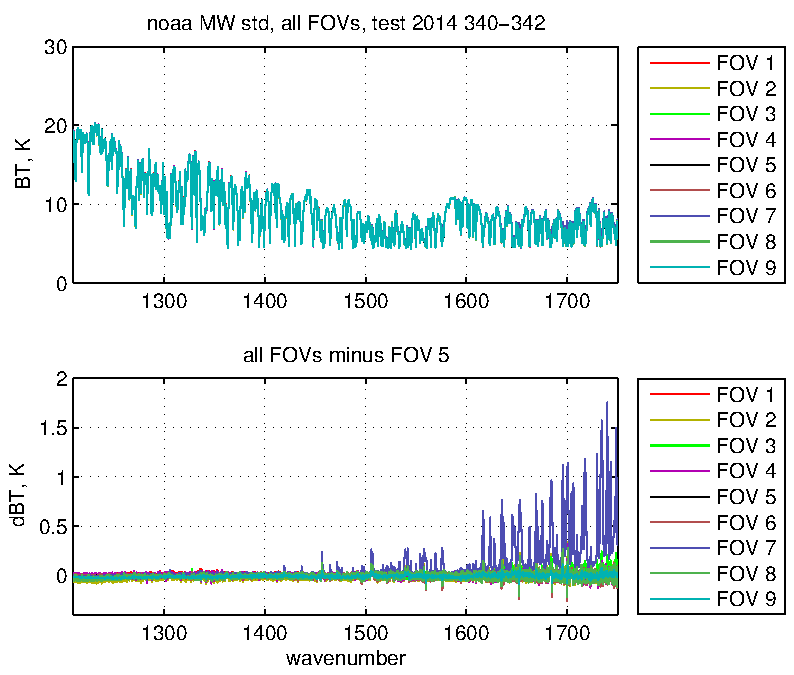
\includegraphics[scale=0.7]{figures/noaa_MW_std_2014_340-342.pdf}
\end{center}

\end{frame}
%----------- slide --------------------------------------------------%
\begin{frame}
\frametitle{ccast SW std}

\begin{center}
  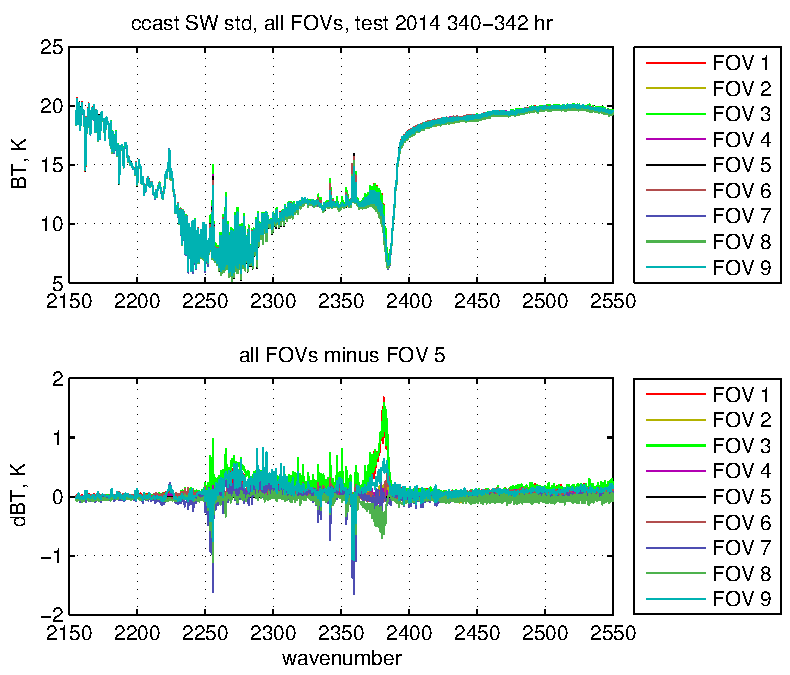
\includegraphics[scale=0.7]{figures/ccast_SW_std_2014_340-342_hr.pdf}
\end{center}

\end{frame}
%----------- slide --------------------------------------------------%
\begin{frame}
\frametitle{noaa SW std}

\begin{center}
  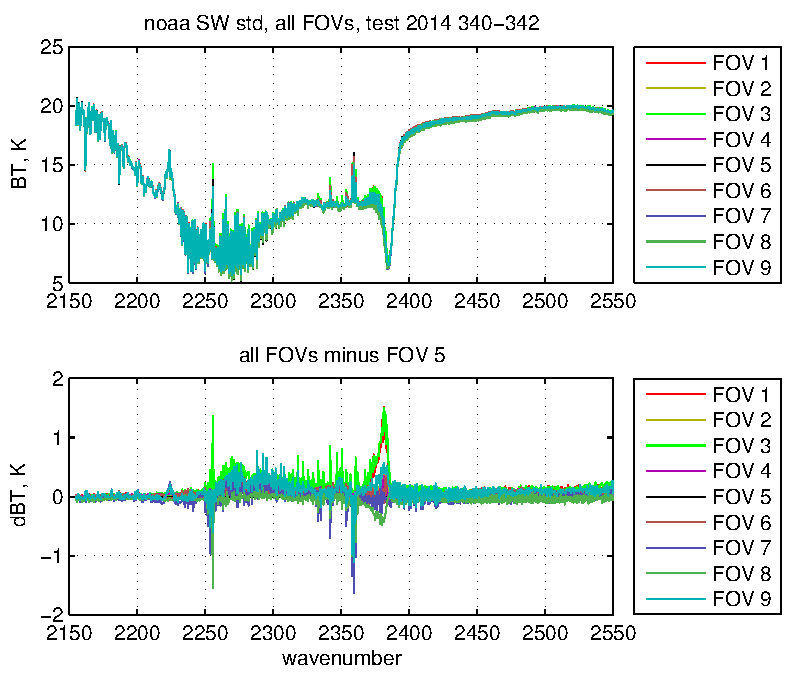
\includegraphics[scale=0.7]{figures/noaa_SW_std_2014_340-342.pdf}
\end{center}

\end{frame}
%----------- slide --------------------------------------------------%
\begin{frame}
\frametitle{calibration equation}

The \ccast\ reference calibration equation is

\[r_{\mbox{\tiny OBS}} = F \cdot r_{\mbox{\tiny ICT}}\cdot f \cdot
  \SA^{-1}\cdot f \cdot \frac{\ES - \SP}{\IT - \SP} \]

\begin{itemize}
  \item $r_{\mbox{\tiny OBS}}$ is calibrated radiance at the user grid
  \item $F$ is Fourier interpolation from sensor to user grid
  \item $f$ is a raised-cosine bandpass filter
  \item $r_{\mbox{\tiny ICT}}$ is expected ICT radiance at the sensor grid
  \item $\SA^{-1}$ is the inverse of the ILS matrix
  \item $\ES$ is earth-scene count spectra
  \item $\IT$ is calibration target count spectra
  \item $\SP$ is space-look count spectra
\end{itemize}

\end{frame}
%----------- slide --------------------------------------------------%
\begin{frame}
\frametitle{calibration notes}

\begin{itemize}

  \item the $\IT$ and $\SP$ looks are averaged over several scans

  \item the UW nonlinearity correction is applied to count spectra
    before application of the calibration equation

  \item as part of the nonlinearity correction we divide the count
    spectra by the numeric filter at the sensor grid, but note this
    cancels out in the ratio $(\ES - \SP) / (\IT - \SP)$

  \item the passband for $f$ is the user grid.  The wings are
    parameters currently set at 15, 20, and 22 \wnum\ for the LW,
    MW, and SW bands

  \item $f \cdot \SA^{-1} \cdot f$ can be considered as a
    physically-based smoothing of the rows and columns of $\SA^{-1}$

  \item $F$ is a zero-filled double Fourier interpolation

\end{itemize}

\end{frame}
%----------- slide --------------------------------------------------%
\begin{frame}
\frametitle{ccast ILS}

the \cris\ \ils\ for $\fov_i$ can be represented as

\[\int_{\mbox{\tiny FOV}_i} \!\!\!\! w_i(\theta)\, \psinc(2 \pi
                 d(v - v_0 \cos \theta ))\, d\theta \]

% f_{v_0}(v) = 
% \int_{\mbox{\tiny FOV}_i}
% \int_{a_i}^{b_i}

\begin{itemize}
  \item $d$ is max \opd
  \item $v$ is frequency
  \item $v_0$ is reference or channel frequency
  \item $\psinc(x) = sin(x)/(n \sin(x/n))$ for $x \ne 0$,  $1$ for
    $x = 0$, where $n$ is the number of points in the sensor grid
   \item $\psinc(2 \pi d(v - v_0 \cos \theta ))$ gives the ILS for a
    single ray at off-axis angle $\theta$
  \item integration is over the intersection of on-axis arcs with
    $\fov_i$, with $w_i(\theta)$ the length of an intersecting arc
    at off-axis angle $\theta$
\end{itemize}

\end{frame}

\end{document}

